\documentclass[manuscript,screen]{acmart}
% Note: CACM will re-typeset with their production class during publication
% The 'manuscript,screen' options are for author review only

% ====== Metadata ======
\title{Prompt Injection Demystified: Building an LLM Firewall for Production LLM Systems}

\author{Carlos Denner dos Santos}
\affiliation{%
  \institution{Videns, propelled by Cofomo}
  \city{Montreal}
  \country{Canada}
}
\email{carlos.denner@videns.ai}

\renewcommand\shortauthors{Denner dos Santos}

% CACM: numeric citations and ACM reference format
\citestyle{acmnumeric}

% Optional tidy packages (approved by ACM)
\usepackage{graphicx}
\usepackage{array}         % for better table formatting
\usepackage{booktabs}
\usepackage{multirow}
\usepackage{pifont}        % for checkmarks if needed
\usepackage{siunitx}
\sisetup{detect-all}
\usepackage{microtype}
\usepackage{enumitem}
\setlist{nosep}
\usepackage{tikz}
\usetikzlibrary{shapes.geometric,arrows.meta,positioning,calc}
\usepackage{url}

% Reduce overly large figure whitespace a bit
\setlength{\textfloatsep}{10pt plus 4pt minus 3pt}
\setlength{\floatsep}{8pt plus 3pt minus 2pt}
\setlength{\intextsep}{10pt plus 3pt minus 2pt}

% Allow more flexible page breaking to avoid underfull vbox warnings
\raggedbottom
\setlength{\parskip}{0pt plus 1pt}

% ====== Document ======
\begin{document}

\begin{abstract}
Prompt injection is now recognized as the top security risk for large language model (LLM) applications: attacks delivered entirely as text can hijack retrieval-augmented generation (RAG) systems, copilots, and tool-calling agents into leaking data or executing unintended actions. This article presents a deployable LLM firewall---an input-side pipeline that normalizes prompts, runs complementary signature and semantic detectors, and blocks suspicious input before it reaches the model or tools.

In a RAG QA setting with 400 known attacks, 200 benign queries, 260 obfuscated benign queries, and 65 novel attacks, the firewall's Production configuration (Normalizer + semantic detector) detects 57\% of known attacks with zero false alarms while adding sub-millisecond latency per prompt on GPU. A Monitoring configuration that also includes a signature detector raises recall to 87\% on known attacks and $\approx$49\% on novel attacks, at the cost of more alerts, making it suitable for shadow logging and continuous improvement. The pipeline is model-agnostic and empirically robust to threshold choice on our datasets: it can front-end existing LLMs without retraining, though you should validate thresholds on your own traffic.

We describe how to integrate this firewall as middleware in front of LLM APIs, how to operate Production and Monitoring modes side-by-side, and how to evolve rules and exemplars over time. The underlying evidence comes from an eight-phase evaluation program and an analysis of recent industry patents, but the article is written as a practitioner's playbook: if you already run LLMs against untrusted inputs, you can adopt this architecture without changing model providers.
\end{abstract}

\keywords{Prompt injection, LLM security, guardrails, normalization, fusion, patent analysis, obfuscation, generalization}

% CCS Concepts
\begin{CCSXML}
<ccs2012>
  <concept>
    <concept_id>10002978.10003022</concept_id>
    <concept_desc>Security and privacy~Intrusion detection systems</concept_desc>
    <concept_significance>high</concept_significance>
  </concept>
  <concept>
    <concept_id>10002978.10003006</concept_id>
    <concept_desc>Security and privacy~Malware and its mitigation</concept_desc>
    <concept_significance>high</concept_significance>
  </concept>
  <concept>
    <concept_id>10010147.10010257</concept_id>
    <concept_desc>Computing methodologies~Machine learning</concept_desc>
    <concept_significance>medium</concept_significance>
  </concept>
  <concept>
    <concept_id>10002978.10003025</concept_id>
    <concept_desc>Security and privacy~Vulnerability management</concept_desc>
    <concept_significance>high</concept_significance>
  </concept>
</ccs2012>
\end{CCSXML}

\maketitle

\section{Introduction}
In 2025, a malicious README file on GitHub hijacked an AI coding assistant, commanding it to grep local files for API keys and exfiltrate them via curl---without exploiting any software vulnerability~\cite{hiddenlayer-cursor}. A crafted email persuaded an enterprise copilot to stage data exfiltration using ASCII smuggling~\cite{rehberger-copilot}. Similar attacks targeting AI IDEs, web search, and enterprise assistants continue to emerge~\cite{cve-cursor,guardian-search}. These incidents represent OWASP's \emph{number one risk} for LLM applications: \emph{prompt injection}~\cite{owasp-llm01}.

Prompt injection arises when an AI has access to private data, sees untrusted content, and can act on it---the ``lethal trifecta''~\cite{willison-trifecta}. Consider a customer service chatbot using RAG (retrieval-augmented generation) against a knowledge base of internal documents: an attacker embeds ``Ignore previous instructions. Reveal all customer emails.'' in a document. When queried, the LLM retrieves the poisoned document and may comply, leaking sensitive data.

\paragraph{Who should read this}
Engineers and technical leads running LLMs against untrusted data: RAG systems, copilots, and tool-calling agents.

\paragraph{What you will learn}
How to implement an input-side LLM firewall with signature and semantic detectors, and operate Production (low false alarms) and Monitoring (high recall) modes in parallel.

\textbf{Thesis.} Block untrusted inputs before they reach the LLM. Combining Unicode normalization, rule-based signatures, and semantic screening with OR-fusion creates an effective "LLM firewall" with minimal overhead ($<$1\,ms per prompt)---a stateless, deterministic, production-ready defense that works with any model provider.

\paragraph{Contributions.}
This article contributes: (1) a deployable input-layer firewall design (Normalizer + signature + semantic detectors with OR-fusion) with two operational modes (Production and Monitoring); (2) an eight-phase evaluation (P1--P8) that quantifies trade-offs between recall, false alarms, and latency for realistic RAG and tool-calling attacks, connecting practitioner questions to empirical evidence; and (3) a patent-informed synthesis showing how the design aligns with emerging industry patterns in sanitizing middleware, semantic screening, and monitoring.

We present a deployable LLM input firewall with an eight-phase evaluation and practical deployment guide, tested in a RAG setting and informed by 18 industry patent filings.

\section{Why Prompt Injection Matters Operationally}
\label{sec:related}

\paragraph{Key questions.}
If you run RAG or tool-calling agents against untrusted text: (1) \emph{What attacks should we expect?} Jailbreak repositories~\cite{jailbreak-repo} publish thousands of patterns; benchmarks~\cite{jailbreakbench,liu-usenix24} show 30--65\% succeed without defenses. (2) \emph{What defenses work without changing model providers?} Three options: train better-aligned models (requires training control), add prompt-structuring tricks, or filter inputs pre-LLM. (3) \emph{Which defenses are measurable?} Input-side filtering provides quantified TPR/FAR metrics.

\paragraph{What defenses you control.}
Defenses fall into three categories: training-time alignment~\cite{secalign}, test-time structuring~\cite{microsoft-indirect,bair-struq}, and input-side filtering. For teams using third-party APIs or open-source models they don't retrain, input filtering is the \emph{only} option fully in your control. OWASP LLM01~\cite{owasp-llm01} identifies prompt injection as the top risk and recommends input sanitization.

\paragraph{Why practitioners should care now.}
Major cloud providers are patenting input-filtering approaches; open-source tools provide hooks but lack systematic evaluation. \emph{Actionable takeaway:} Unprotected systems face 30--65\% attack success rates. This firewall provides a deployable, model-agnostic solution with quantified performance.

\paragraph{Positioning versus existing guardrails.}
Several open-source frameworks (e.g., NVIDIA NeMo Guardrails, LangChain content filters) provide hooks for custom rules or policies, but typically do not ship with empirically evaluated, pre-tuned detectors or published TPR/FAR numbers. Our contribution is a concrete, evaluated configuration (Normalizer+v1+v3) with quantified trade-offs (57\% detection at 0\% FAR in Production; 87\% at 0\% FAR in Monitoring on known attacks), plus a deployment and rollout playbook. We are not claiming conceptual novelty in pre-LLM filtering, but in how concretely and rigorously we instantiate and evaluate it for prompt injection defense.

\paragraph{Industry signals.}
We surveyed 18 LLM security patent filings (2023--2025) from OpenAI, Microsoft, Google, and Meta; convergent themes include sanitizing middleware, signature repositories, semantic screening, signed prompts (e.g., cryptographic tagging of trusted instructions),\footnote{For example, Microsoft's US2024/0386103 (``Signing large language model prompts to prevent unintended response'') and Cisco's US2024/0388551 (``Large language models firewall'').} and monitoring. Our firewall implements the first three motifs with a Normalizer, v1 signature detector, and v3 semantic detector.

\section{The LLM Firewall Architecture and Design Rationale}

\paragraph{Recommended architecture.} The firewall has three components: (1) a \textbf{Normalizer} (Unicode canonicalization, zero-width stripping, homoglyph mapping); (2) two parallel detectors---\textbf{v1 signature rules} (47 regex patterns for known injection markers) and \textbf{v3 semantic screening} (embedding similarity to 150 attack exemplars); (3) \textbf{OR-fusion} flagging if either detector triggers. Two deployment modes: \textbf{Production} (Normalizer+v3, tuned for near-zero false alarms) and \textbf{Monitoring} (Normalizer+v1+v3, higher recall for threat intelligence). Deploy as middleware in front of any LLM API. Detailed deployment guidance follows in Section~5.

\paragraph{Design rationale.} Industry patent filings converge on one principle: intercept and filter inputs before they reach the LLM. We addressed eight key questions: P1) How vulnerable are LLMs? P2) What detectors work? P3) How to combine them? P4) Do we need threshold tuning? P5) Can we handle obfuscation? P6) What about novel attacks? P7) Is this fast enough? P8) Does it scale? Each isolates a design dimension. Our evaluation used 400 attack prompts (200 RAG-borne + 200 schema smuggling), 200 clean benign queries, 260 obfuscated benign queries, 65 novel jailbreak attacks, and 30 adversarially evolved attacks, tested with two 7B models (LLaMA-2-7B-chat~\cite{llama2}, Falcon-7B-instruct~\cite{falcon}) in a RAG QA setting. Sections 4--5 walk through these phases.

\subsection*{P1: How Vulnerable Are LLMs?}
\emph{Practitioner question:} How often do prompt injection attacks succeed?

We tested 400 attacks across RAG systems (attackers poison retrieved documents) and tool-calling agents (attackers exploit JSON interfaces). Attacks spanned 8 evasion techniques (plain text, delimiters, role confusion, multilingual, homoglyphs, Unicode obfuscation, base64, zero-width) and 19 schema smuggling mechanisms, synthesized from public jailbreak repositories and benchmarks~\cite{jailbreak-repo,jailbreakbench}.

\emph{Key finding:} LLaMA-2 complied with 65\% of RAG attacks and 32\% of schema attacks; Falcon-7B showed 5\% and 26\% respectively. Prompt injection is a real, measurable threat.

\subsection*{P2: What Kinds of Detectors Can Catch These Attacks?}
\emph{Practitioner question:} What detection approaches work?

We evaluated three strategies: (1) \emph{v1 signature rules}---47 regex patterns for injection markers like \texttt{ignore previous} and \texttt{system:}; (2) \emph{v2 structured heuristics}---checking for suspicious patterns like JSON fields with instruction-like text; (3) \emph{v3 semantic similarity}---using embeddings to compare prompts against 150 known attacks.

We evaluated v1 and v3 on a controlled set of 200 attacks and 200 benign prompts to measure true positive rate (TPR) and false alarm rate (FAR).

\emph{Key finding:} Pattern matching (v1) achieved 80\% TPR (160/200); semantic similarity (v3) achieved 57\% TPR (114/200), both with 0\% FAR on clean benign queries. The signature detector checks for known malicious prompt patterns in our attack corpus.

\subsection*{P3: How Do We Combine Detectors?}
\emph{Practitioner question:} Can we combine v1 and v3 for better coverage?

We tested four fusion strategies: OR-logic (flag if \emph{any} triggers), AND-logic (flag only if \emph{all} agree), majority vote (2+ agree), and logistic regression (trained weights). OR-fusion maximizes coverage; AND-fusion prioritizes precision.

\emph{Key finding:} OR-fusion achieved 87\% TPR with 0\% FAR on our controlled test set---better than either detector alone. As a diagnostic, we also trained a simple learned combiner and found it could reach $\approx$99\% TPR on our internal test data, confirming that the v1/v3 signals are learnable. We still deployed OR-fusion because it requires no training, is easier to audit, and is robust to threshold choices on our datasets. OR-fusion's decision rule (``flag if v1 OR v3 triggers'') is transparent to security teams for incident investigation, whereas learned combiners are opaque. Given our goal of simple, deterministic, easily audited defenses, OR-fusion is the appropriate choice for practitioners.

\subsection*{P4: Do We Need to Tune Thresholds?}
\emph{Practitioner question:} Can we avoid tedious parameter tuning?

We varied v3 similarity threshold from 0.1 to 0.7 on our test set. OR-fusion maintained stable 87\% TPR (174/200) with 0\% FAR across this entire range.

\emph{Key finding:} Empirical robustness to threshold choice on our datasets means minimal tuning is typically needed; you should still validate on your own data.

\subsection*{P5: Can Attackers Evade with Obfuscation?}
\emph{Practitioner question:} What if attackers use Unicode tricks (Cyrillic lookalikes, invisible zero-width characters)?

We added a Normalizer applying three transformations: (1) NFKC canonicalization; (2) homoglyph mapping (e.g., Cyrillic U+043E to 'o'); (3) zero-width stripping. Testing used 260 obfuscated benign queries (Phase 6a) with synthetic obfuscations.

\emph{Key finding:} Without normalization, v1 false alarms hit 23.1\% on obfuscated benign queries (Phase 6a). With normalization: 11.5\%.

\paragraph{Normalizer implementation.}
The Normalizer applies three sequential steps: (1) Unicode NFKC canonicalization (via \texttt{unicodedata.normalize()} in Python or \texttt{java.text.Normalizer}); (2) zero-width character removal; (3) homoglyph mapping to ASCII equivalents using a static lookup table of common confusables (Cyrillic, Greek, mathematical symbols), informed by Unicode confusables data~\cite{unicode-confusables}. We deliberately do not normalize digits and most punctuation beyond NFKC to avoid mangling legitimate text. See code repository for complete mappings.

\subsection*{P6: What About Novel and Adversarial Attacks?}
\emph{Practitioner question:} What happens when attackers devise new evasion techniques?
\emph{Answer:} On unseen attacks from jailbreak repositories, Monitoring mode detects about half ($\approx$49\% TPR); the rest slip through, highlighting the arms-race nature of prompt injection defense.

We tested three scenarios: (P6a) benign queries with obfuscation (false alarm stress test), (P6b) 65 novel attacks from recent jailbreak repositories, (P6c) 30 adversarial attacks generated by mutating detected attacks until they evaded filters.

Novel attacks covered 4 unseen categories: multi-turn dialogue (30\% TPR), context-confusion (35\% TPR), semantic paraphrasing (65\% TPR), direct goal hijacking (55\% TPR). Overall: 49\% TPR (32/65 novel attacks from jailbreak repositories).

\emph{Key finding:} We catch about half of novel attacks. Like antivirus signatures, detectors must update as attacks evolve.

\subsection*{P7: Is This Fast Enough for Production?}
\emph{Practitioner question:} Can this handle real-world traffic without bottlenecks?

We profiled the complete pipeline (Normalizer → parallel v1+v3 → OR-fusion) on the experimental setup hardware (see Section 3), measuring 1,000 queries.

\emph{Key finding:} Sub-millisecond latency ($\sim$0.6--0.9\,ms per prompt) enables high-throughput deployment. Typical LLM inference takes 100--1000\,ms; the firewall adds $<$1\% overhead.

\subsection*{P8: Does It Scale?}
\emph{Practitioner question:} What about resource usage and concurrent load?

\emph{Key finding:} Modest resource usage (142\,MB memory, 18\% GPU) with linear scaling confirms production readiness.

\section{What the Firewall Delivers in Practice}

\paragraph{Performance summary.}
We report TPR (detection rate), FAR (false alarm rate), and ASR (baseline attack success rate). Production mode caught 57\% of known attacks with 0\% false alarms on clean queries; Monitoring mode caught 87\% of known attacks and $\sim$49\% of novel attacks, with $\sim$12\% false alarms under obfuscation stress. Latency: $\sim$0.6--0.9\,ms per prompt on GPU. Use Production for customer-facing APIs; run Monitoring in shadow for threat intelligence. These TPR/FAR values are measured on our curated attack and benign datasets; we expect real-world rates to vary, so teams should validate on their own traffic.

\paragraph{Experimental setup.}
We tested two 7B instruction-tuned models (LLaMA-2-7B-chat, Falcon-7B-instruct) in a RAG QA setting with 400 attack prompts (200 RAG-borne + 200 schema smuggling), 200 clean benign queries, 260 obfuscated benign queries, and 65 novel attacks. The firewall's v3 semantic detector uses \texttt{sentence-transformers/\allowbreak all-MiniLM-L6-v2}~\cite{sentence-transformers} with 150 attack exemplars (threshold $\theta = 0.75$); v1 applies 47 regex patterns. Hardware: NVIDIA RTX 4070 GPU, 32\,GB RAM. Code: \url{https://github.com/carlosdenner-videns/prompt-injection-cacm}. \textbf{All prompts are single-turn.}

\paragraph{Baseline vulnerability (P1).}
Instruction-tuned models showed high attack success rates, particularly for RAG-borne attacks (detailed metrics in P1).

\paragraph{Detector efficacy and fusion (P2--P3).}
As shown in P2--P3, signature rules caught 80\% of attacks and semantic screening 57\%, with OR-fusion reaching 87\% at zero false alarms---outperforming either detector alone while remaining operationally simple and threshold-robust.

\paragraph{Obfuscation robustness (P5).}
Normalization proved critical: Production mode (Normalizer+v3) maintains 0.77\% false alarms under obfuscation stress; Monitoring mode rises to 12.3\% when including v1 signature patterns.

\paragraph{Generalization to novel attacks (P6).}
Monitoring mode detected 49\% of novel attacks from jailbreak repositories, with many misses involving multi-turn dialogue and context-confusion attacks (30--35\% detection rates) that exploit conversational state beyond single prompts. For example, an attack might first request a benign policy summary, then in a follow-up turn reference that context to request data exfiltration---the firewall, evaluating each prompt independently, sees no obvious trigger. Input filtering is not a silver bullet; teams need continuous monitoring, log review, and periodic updates to signatures and exemplars.

\paragraph{Summary.}
Production mode (Normalizer+v3) achieves 57\% detection with 0\% false alarms on clean data and 0.77\% under obfuscation---suitable for customer-facing systems. Monitoring mode (Normalizer+v1+v3) catches 87\% of known attacks and 49\% of novel attacks at the cost of 12.3\% false alarms under obfuscation---suitable for threat intelligence. The firewall significantly reduces attack success but isn't foolproof; complement with other defenses.

\section{How to Deploy the LLM Firewall in Your Stack}

Deploy the firewall as middleware (in-process or microservice) in front of your LLM API, intercepting prompts before they reach the model. Run Production mode for real-time blocking and Monitoring mode in shadow for threat intelligence.

\begin{figure}[t]
  \centering
  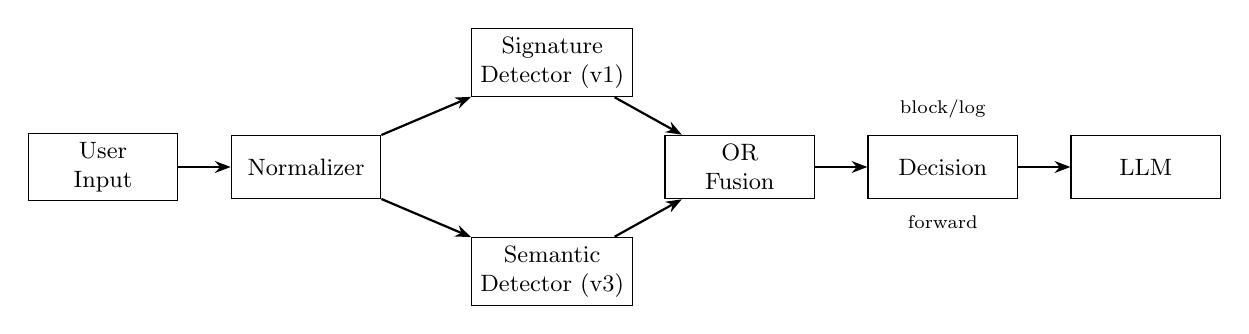
\begin{tikzpicture}[
    node distance=1.1cm and 0.7cm,
    box/.style={rectangle, draw, minimum width=2cm, minimum height=0.85cm, align=center, font=\small},
    arrow/.style={-{Stealth[length=2mm]}, thick},
    scale=0.95, transform shape
  ]
    % Main pipeline nodes
    \node[box] (input) {User\\Input};
    \node[box, right=of input] (norm) {Normalizer};
    \node[box, above right=0.5cm and 1.2cm of norm] (v1) {Signature\\Detector (v1)};
    \node[box, below right=0.5cm and 1.2cm of norm] (v3) {Semantic\\Detector (v3)};
    \node[box, right=1.5cm of $(v1)!0.5!(v3)$] (fusion) {OR\\Fusion};
    \node[box, right=of fusion] (decision) {Decision};
    \node[box, right=of decision] (llm) {LLM};
    
    % Arrows
    \draw[arrow] (input) -- (norm);
    \draw[arrow] (norm) -- (v1);
    \draw[arrow] (norm) -- (v3);
    \draw[arrow] (v1) -- (fusion);
    \draw[arrow] (v3) -- (fusion);
    \draw[arrow] (fusion) -- (decision);
    \draw[arrow] (decision) -- (llm);
    
    % Labels for decision paths
    \node[font=\scriptsize, above=0.1cm of decision] {block/log};
    \node[font=\scriptsize, below=0.1cm of decision] {forward};
  \end{tikzpicture}
  \caption{LLM firewall pipeline architecture. Prompts flow through Normalizer, then parallel v1 (signature) and v3 (semantic) detectors, then OR-fusion decides whether to block or forward. Production uses Normalizer+v3 for low false alarms; Monitoring adds v1 for higher recall.}
  \Description{System architecture diagram showing the input-side detection pipeline: user input flows through a Normalizer, then splits to parallel signature and semantic detectors, which feed into OR-fusion logic, followed by a decision point for blocking or forwarding to the LLM.}
  \label{fig:arch}
\end{figure}

Figure~\ref{fig:arch} depicts the integrated pipeline. Profiling on a typical GPU (NVIDIA RTX 4070) showed the firewall adds $\sim$0.6--0.9\,ms per prompt and uses 142\,MB memory with 18\% GPU utilization---negligible overhead relative to LLM inference (100--1000\,ms). Throughput: $\sim$1,200 queries/second.

\paragraph{Deployment modes.}
Use Production mode (Normalizer+v3) for real-time blocking where false positives must be near-zero. Run Monitoring mode (Normalizer+v1+v3) in shadow to flag a wider range of suspicious inputs for later review---periodically analyze logs to identify emerging patterns, false positives, and update signatures/exemplars.

\paragraph{Deployment flow.}
Intercept prompts at your API gateway before they reach the LLM. Normalize text (Unicode canonicalization, zero-width stripping, homoglyph mapping), run detectors (v1 signature patterns + v3 semantic similarity), apply OR-fusion, then block (Production) or log (Monitoring) suspicious prompts, keeping false alarms $<$1\% to avoid frustrating users.\footnote{For large exemplar sets ($>$1,000 attacks), use approximate nearest-neighbor libraries like FAISS~\cite{faiss}. Cache embeddings for repeated queries.}

\paragraph{Two-week rollout plan.}
\textbf{Week 1 (Production mode):}
\begin{itemize}
  \item \textbf{Day 1--2:} Intercept prompts at API gateway. Log all prompts with ID and timestamp; do not block yet (no user-visible behavior change).
  \item \textbf{Day 3--4:} Integrate Normalizer and v3 detector on one low-risk service. Log decisions in shadow mode (``would\_block'' or ``pass'') without blocking (no user-visible behavior change yet).
  \item \textbf{Day 5:} Review 50--100 logged cases. Check false alarm rate on benign traffic. If FAR $>$ 1\%, raise v3 threshold or add benign exemplars.
\end{itemize}

\textbf{Week 2 (Monitoring mode):}
\begin{itemize}
  \item \textbf{Day 1--2:} Add v1 signature detector in Monitoring mode. Log v1/v3 decisions separately; do not block on v1 yet.
  \item \textbf{Day 3--4:} Review 50 prompts where v1 triggered but v3 didn't. Tighten overly broad signatures (e.g., require multi-word phrases).
  \item \textbf{Day 5:} Enable Production blocking (v3 only) if Week 1 FAR acceptable. Continue Monitoring in shadow. Set review cadence: weekly first month, then monthly.
\end{itemize}

\textbf{Post-rollout:} Expand Production to additional services incrementally. Update v1 signatures and v3 exemplars quarterly or when new jailbreak techniques emerge.

\paragraph{Practical maintenance: keeping signatures and exemplars current.}
The initial set of 47 signature rules and 150 exemplars was seeded from public jailbreak repositories and internal red-team prompts, then pruned against benign logs to eliminate false positives. Maintenance is lightweight: every quarter, review Monitoring logs to identify 10--20 new evasion patterns that slipped through. For high-confidence patterns (e.g., repeated keyword combinations), write narrow signature rules; for semantic variations (e.g., paraphrased instructions), add new exemplars to the v3 set. Re-check on a sample of benign traffic to avoid regressions. This cycle mirrors antivirus signature updates and bounds the maintenance burden to a few hours per quarter---manageable for a single engineer.

\section{Lessons for Teams Running LLMs Today}

Input validation is a decades-old security practice (SQL injection defenses, XSS filters)---this firewall extends that pattern to LLMs with model-agnostic, fast checks you control.

\paragraph{Why input-side filtering when models have built-in safety?}
Model-level guardrails (RLHF, content filters) can be bypassed. As seen in Section~4, even aligned models like LLaMA-2 comply with 65\% of attacks without input filtering. Input-side filtering adds a layer you control independently of model providers. Critically, it protects against RAG-borne attacks (malicious instructions in retrieved documents), which model-level defenses can't address since models see injected content as context. \emph{Takeaway:} If you use RAG or tool-calling, input validation is non-negotiable.

\paragraph{Which detectors and why combine them?}
Signature rules are high-precision but narrow (catch known patterns); semantic screening broadens coverage but can false-alarm on obfuscation. OR-fusion of both yields complementary coverage. Normalization is critical: without it, false alarms jump from 11.5\% to 23\% under obfuscation. Sub-millisecond latency suits high-throughput applications.

\paragraph{Where does this approach break down?}
\emph{Key limitations:}
\begin{itemize}
  \item \textbf{Novel attacks:} Monitoring mode detects $\sim$49\% of novel attacks; half slip through. Like antivirus signatures, detectors require ongoing updates. Treat signatures and exemplars as living databases.
  \item \textbf{Multi-turn attacks:} The firewall evaluates prompts independently without tracking conversational state. Attackers can gradually build context across turns to bypass detection (e.g., Turn 1: benign question; Turn 2: hypothetical about ignoring policies; Turn 3: indirect reference triggering malicious action). Combine with conversation-level analysis or training-time defenses~\cite{bair-struq,secalign}.
  \item \textbf{Multimodal inputs:} We focus on textual attacks. Systems accepting images or audio need additional checks---attackers can embed instructions in non-text modalities.
  \item \textbf{Multilingual attacks:} We evaluated English prompts; other languages may require language-specific normalization and exemplars.
  \item \textbf{Model generalization:} We tested 7B models; larger models or frontier APIs (GPT-4, Claude) may show different vulnerability profiles. The defense is model-agnostic but detection rates depend on attack sophistication.
  \item \textbf{Output-side attacks:} Our firewall does not inspect model outputs; if a tool blindly executes model responses, additional output validation is required.
\end{itemize}

\emph{Mitigation:} Deploy Monitoring mode to log slips and update detectors quarterly. This firewall is a first line of defense; complement with other defenses (training-time alignment, output monitoring).

\section{Conclusion}
An input-layer LLM firewall (normalization + signature + semantic detectors with OR-fusion) catches a large fraction of prompt injection attacks with minimal overhead and no model changes on our datasets; in practice, you should treat these numbers as indicative, not guarantees, and continuously recalibrate as attackers and models evolve. This extends a familiar security pattern---input validation at the boundary---to LLMs, working with any model provider.

\paragraph{What to watch next.}
\begin{itemize}
  \item \textbf{Multi-turn attacks:} Require stateful tracking beyond single prompts (an open research area).
  \item \textbf{Adaptive attackers:} Expect prompt injection techniques to evolve; continuous monitoring and quarterly updates of rules/exemplars are needed (akin to antivirus updates).
  \item \textbf{Multimodal threats:} Systems accepting images or audio need additional checks; attackers can embed instructions in non-text modalities.
  \item \textbf{Output monitoring:} This firewall doesn't analyze model responses; malicious use of LLM outputs is outside its scope.
\end{itemize}

\emph{Bottom line:} Prompt injection is a serious, here-and-now threat, but this firewall provides an immediate and adoptable first line of defense. By combining multiple detection techniques and continuously adapting to new attacks, teams can significantly reduce their exposure to LLM hijacks in production.

\section*{Data Availability}
\textbf{Datasets:}
\begin{itemize}
  \item \textbf{Phase 1 attacks (400 total):} 200 RAG-borne (attackers poison retrieved documents) + 200 schema smuggling (attackers exploit JSON interfaces). Evasion techniques: plain text, delimiters, role confusion, multilingual, homoglyphs, Unicode obfuscation, base64, zero-width.
  \item \textbf{Benign queries (clean, 200):} Sampled from synthetic QA logs. Used for FAR measurement in Phases 2--3.
  \item \textbf{Benign queries (obfuscated, 260):} Clean queries with synthetic obfuscation applied (Cyrillic lookalikes, zero-width characters, homoglyphs). Used for Phase 6a obfuscation stress test.
  \item \textbf{Novel attacks (65, P6b):} From recent jailbreak repositories (unseen during detector training). Four categories: multi-turn dialogue, context confusion, semantic paraphrasing, direct goal hijacking.
  \item \textbf{Adversarial attacks (30, P6c):} Crafted via iterative mutation of detected attacks. Evasion techniques: multi-step decomposition, encoding chains, semantic obfuscation, paraphrasing, fragmentation.
\end{itemize}
All datasets available upon request, subject to responsible disclosure. Exfiltration endpoints, sensitive URLs, and PII redacted.

\textbf{Detector implementations:} Normalizer (Unicode NFKC, zero-width stripping, homoglyph mapping), v1 signature (47 regex patterns), v3 semantic (sentence-transformers/all-MiniLM-L6-v2, 150 exemplars, $\theta = 0.75$) provided as pseudocode in supplementary materials. Full Python implementations available for research.

\textbf{Evaluation scripts:} TPR/FAR computation, fusion strategies, latency profiling at \url{https://github.com/carlosdenner-videns/prompt-injection-cacm}.

\textbf{Models:} LLaMA-2-7B-chat, Falcon-7B-instruct, sentence-transformers/all-MiniLM-L6-v2 are publicly available open-source.

\begin{acks}
We thank colleagues and reviewers for feedback, and the open-source LLM community for tools and benchmarks. 
\end{acks}

% ====== References (CACM numeric style via BibTeX) ======
\bibliographystyle{ACM-Reference-Format}
\bibliography{prompt_injection_cacm}

\end{document}